%  公立はこだて未来大学 卒業論文 テンプレート ver1.50
% (c) Junichi Akita (akita@fun.ac.jp), 2003.10.31
% update by N.T.,  2004.11.10
%
\documentclass{funthesis}
%\documentclass[english]{funthesis} % use [english] option for English style
\usepackage[dvipdfmx]{graphicx}%図としてpdfの宣言
\usepackage{mediabb} %図としてpdfの宣言
\usepackage{graphicx} % 図(EPS形式)を本文中で読み込む場合はこれを宣言
\usepackage{comment}
\usepackage{float}
% この部分に,タイトル・氏名などを書く.
% タイトルなどの定義の始まり
\jtitle{分散バージョン管理システムGitを用いた
\\ソフトウェア開発者の特徴抽出手法の提案\\
}  % 論文の和文タイトル
%
\etitle{A Proposal of the Method to Characteristic Extraction of Software Developer Using Distributed Version Control System Git
\\
}% 論文の英文タイトル
%
\htitle{A Proposal of Characteristic Extraction Method of Software Developer}   % ヘッダー用の論文の短縮英文タイトル
%     必ず1行に収まるように英文タイトルを短縮する.
%
\jauthor{黒瀬 丈哉}     % 氏名(日本語)
\eauthor{Takeya Kurose}   % 氏名(英語)
\jaffiliciation{情報アーキテクチャ学科} % 所属学科名(日本語)
\eaffiliciation{Department of Media Architecture} % 所属学科名(英語)
\studentnumber{1014154}   % 学籍番号
\jadvisor{伊藤 恵}    % 正指導教員名(日本語)
\eadvisor{Kei Ito}  % 正指導教員名(英語)
\jdate{2018年1月29日}    % 論文提出日   (日本語)
\edate{January 29, 2018}     % 論文提出年月 (英語)
% タイトルなどの定義の終わり

\begin{document}

%--------------------------------------------------------------------
\maketitle       % タイトルページを作成
%--------------------------------------------------------------------
% 英文概要(250語程度)
\begin{eabstract}
In recent years, along with the spread of use of distributed version management system in software development, various software development projects are being shared and managed. As a typical example of such collaborative development tools on the Web, GitHub which is a service using distributed version management system Git can be cited. The development history of GitHub has data of many developers, from there various characteristic of developers can be obtained. In this research, I propose a characteristic extraction method of developers using distributed version control system Git, which aims to analyze and extract characteristics of such software developers' roles and abilities. By analyzing the characteristics of developers extracted by the proposed method, it is expected to utilize in human resources development and human resource evaluation in development projects. In this paper, I describe the outline of proposed characteristic extraction method, the result of experiment using method and its consideration.
\end{eabstract}

% 英文キーワード(5個程度をコンマ(,)で区切って羅列する)
\begin{ekeyword}
Git, GitHub, Characteristic Extraction, Software Developer, Development History\end{ekeyword}

%--------------------------------------------------------------------
% 和文概要(400字程度)
\begin{jabstract}
近年,ソフトウェア開発における分散バージョン管理システムの普及に伴い,様々なソフトウェア開発プロジェクトが共有・管理されるようになっている.こういったWeb上での共同開発ツールの代表例として,分散バージョン管理システムGitを用いたサービスであるGitHubが挙げられる.GitHubの開発履歴には多くの開発者のデータがあり,そこから開発者の様々な特徴を得ることができる.本研究では,このようなソフトウェア開発者の役割や能力に関する特徴を分析し抽出することを目的とした,分散バージョン管理システムGitを用いた開発者の特徴抽出手法を提案する.提案方式によって抽出した開発者の特徴を分析することにより,開発プロジェクトにおける,人材配置や人材評価への活用などが期待される.本稿では,提案する特徴抽出手法の概要や,手法を用いた実験の結果とその考察について述べる.
\end{jabstract}

% 和文キーワード(5個程度をコンマ(,)で区切って羅列する)
\begin{jkeyword}
Git,GitHub,特徴抽出,ソフトウェア開発者,開発履歴
\end{jkeyword}

%--------------------------------------------------------------------
\tableofcontents % 目次を作成


% 本文のはじまり
%--------------------------------------------------------------------
\chapter{序論} % 章のタイトル
%\chapter{Introduction} % sample of English style

% \includegraphics[width=??cm]{hoge.eps} % 図(EPS形式)を読み込む場合

\section{背景} % sectionのタイトル

% 以下に背景,関連する環境,状況,技術に関する概要を記述.

近年,ソフトウェア開発における分散バージョン管理システムの普及に伴い,様々なソフトウェア開発プロジェクトがWeb上で共有・管理されるようになっている.こういったWeb上での共同開発ツールの代表例としてGitHub\cite{GitHub}が挙げられる.
\\ GitHubの開発履歴には多くの開発者のデータがあり,そこから開発者の様々な特徴を得ることができると考えられる.実際にOnoue等の研究では,ソフトウェア開発履歴の分析を行うことにより,開発者には異なる特徴があることが明らかになっている\cite{Onoue_English}.また,GitHubがGitプロジェクトのソースコード・リポジトリを分析するために提供しているGitHub API\cite{GitHub_API}の普及により,オンライン上でのソフトウェア開発に関する様々な解析が盛んに行われるようになっている\cite{Characteristic}.
\section{研究方針}

こういった背景から,本研究では,GitHub上でのソフトウェア開発者の役割やスキルに関する特徴を分析することを目的とした,特徴抽出手法を提案する.そして,提案手法によって抽出した開発者の特徴を分析する.分析結果の活用の例として,開発プロジェクトにおける人材配置や人材評価への活用が挙げられる.
\\ 本研究では,分析対象のデータとしてGitHubで活動している開発者の活動履歴を用いる.そして実際のGitプロジェクトを対象とした実験を行い,実験結果の考察を行う.
\section{論文構成}
本節では次章以降の構成について述べる.まず本稿の第2章では本研究で用いる分散バージョン管理システムGitについて述べる.第3章ではGitを用いて特徴抽出を行なった関連研究についてまとめ,本研究の目標を述べる.第4章では提案する特徴抽出手法の概要について述べる.第5章では提案手法を用いる実験対象や,実験方法,そして実験の結果について述べる.最後に本稿をまとめ,今後の展望について述べる.
%--------------------------------------------------------------------
%--------------------------------------------------------------------
\chapter{分散バージョン管理システム} % 章のタイトル
%\chapter{Introduction} % sample of English style

本章では,本研究で用いるツールである,分散バージョン管理システムGitと,GitホスティングサービスGitHubについての説明を行う.

% \includegraphics[width=??cm]{hoge.eps} % 図(EPS形式)を読み込む場合

\section{Git} % sectionのタイトル

% 以下に背景,関連する環境,状況,技術に関する概要を記述.

Gitは,ソースコード・バージョン管理システム(以下,VCS)に分類されるツールである.Subversionのような,1つのリポジトリを共有する集中型VCSと異なり,Gitは各開発者がソースコードのリポジトリを共有し,リポジトリへの変更内容のみをやりとりするという分散型のVCSとなっている.各開発者が独立したリポジトリを用いて開発を進められることや,ソースコードの変更の責任所在とその履歴管理が容易であるという特徴から,多くのオープンソース開発プロジェクトでGitが利用されている.
\\ Gitでは,ソースコードに対する変更を,コミットと呼ばれる作業でリポジトリに変更する.コミットで登録される情報には,ソースコードへの変更差分に加えて,コミットを行なったユーザーの名前,コミット日時,コミット内容を示す文章が含まれる.各開発者に登録されたコミットは,プロジェクトの中心リポジトリへコミットを組み入れること(以下,マージ)により,分散開発されたコードが一つのソフトウェアとして統合される.リポジトリに登録されたコミットは,その登録順に整列したリストとして管理される.一連のコミット列の途中から異なるコミット列を適用するバージョンを作ることができる.この分岐操作をブランチと呼ぶ.リポジトリ作成時に存在するブランチをマスターブランチと呼び,マスターブランチ以外のブランチは,開発中の一時的な用途として作成され,最終的にマスターブランチへマージする運用が一般的である\cite{Matsubara}.
\section{GitHub}

現在では,クラウドベースでGitリポジトリを提供するサービスが登場しており,GitHubは,Gitリポジトリのホスティングサービスとして広く採用されている.GitHubを用いた分散開発では,各開発者がメインリポジトリを複製(クローン)したリポジトリ上で開発を行い,その後,メインリポジトリのマスターブランチに対する変更履歴のマージを要求するというプロセスが用いられることが多い(図2.1).このプロセスに沿った分散開発では,メインリポジトリのマスターブランチに統合されたコードが最終成果物となる\cite{Matsubara}.
\begin{figure}[H]
\centering  % 図を真ん中に配置
\includegraphics[clip,width = 12cm,height=10cm]{figures/github.pdf}
\caption{分散バージョン管理システムGitHubの概要}    \label{sample}
\end{figure}
\subsection{GitHub API}
GitHub APIはGitHub社が提供しているAPI(以下,GitHub API)であり,Gitプロジェクトのソースコード・リポジトリを分析することに適している\cite{GitHub_API}.図2.2はGitHub APIで取得ができる項目について示している.プロジェクトに携わっている開発者の名前や,概要,プロジェクトオーナーの詳細など様々な項目をプロジェクトごとに取得することが可能である.例えば,「開発プログラミング言語とその使用量」に着目して統計データを取ることで,人気なプログラミング言語をランキング形式でソートし抽出することができる.また,「コミット時のコメント」を分析することで,開発者の感情抽出を行う試みなどがある.
\begin{figure}[H]
\centering  % 図を真ん中に配置
\includegraphics[clip,width=12cm,height=7cm]{figures/github_api.pdf}
  \caption{GitHub APIで取得ができる項目}    \label{sample}
\end{figure}
\chapter{関連研究}
本章では,本研究の関連研究について述べる.3.1節では開発履歴からソフトウェア開発者の分類を行なった先行研究を3つ述べる.3.2節では関連研究のまとめを述べ,本研究の方針を述べる.
\section{開発履歴を用いた関連研究}
\subsection{GitHub上の活動履歴分析による開発者分類}
尾上等は,GitHub 上の活動履歴分析による開発者分類手法の提案を行い,GitHubで活発な OSS(Open Source Software)プロジェクトである homebrewとnode に参加するソフトウェア開発者を活動履歴からクラスタリングし,その結果に基づいて開発者の分類を行った\cite{Onoue_Japan}.分析の結果,活動内容や活動の活発さから開発者が5つのクラスタに分類されることが明らかになった.一方で,開発者の能力や役割に関わる特徴を抽出することに関しての研究は行われていなかった.
\subsection{分散バージョン管理システムの共同開発履歴に基づいた開発者の特徴抽出手法の検討}
李等はソフトウェア開発者の役割やスキルに関する特徴を分析することを目的とした,分散ソースコード管理システムの共同開発履歴に基づいた開発者の特徴抽出手法について分析した\cite{risyo}. 提案方式として,プロジェクトにおける開発者の3つの観点において特徴の抽出を行うことで,提案方式の実現可能性を検証した.この提案方式はプロジェクト全体における開発者の特徴を抽出しており,開発箇所における開発者の特徴を抽出する研究は行われてはいなかった.
\subsection{開発履歴を利用した風林火山モデルに基づく開発者特性の分析}
五田等は開発者特性を定量的に分析するために,ソフトウェアのプロジェクト管理とバグ追跡のためのツールであるTracや,集中型バージョン管理システムSubversionの開発履歴を基に,ソフトウェア開発者の能力分類を行う手法を提案した.\cite{gota}.提案方式として,「風,林,火,山」で特徴付けされた4つの能力に,測定したメトリクスを割り当てて,それぞれの能力値を客観的に表すモデルの提案を行った.ケーススタディといて,大学院生を対象としたScrumの開発演習からメトリクス値を算出し,受講生49名の能力値を算出した.課題点として,GitではなくSubversionの開発履歴から,ソフトウェア開発者の特性の分析を行なった点が挙げられる.図3.1は世界でのGit(青線)とSubversion(赤線)の注目度(Google検索数)を示すグラフである\cite{google_trends}.2008年ごろを境にSubversionとGitの注目度が逆転し、Subversionは下火に,一方のGitの注目度はうなぎのぼりという状況となっている.より関心が持たれているGitの開発履歴を対象とすることで,提案手法の有用性が確保できると考えられる.
\begin{figure}[H]
\centering  % 図を真ん中に配置
\includegraphics[clip,width=14cm]{figures/git_subversion.pdf}
  \caption{GitとSubversionの注目度の動向}    \label{sample}
\end{figure}
\section{まとめ}
上記で述べた3つの関連研究の課題点から,本研究では,GitHub上の開発履歴から,ソフトウェア開発者の開発箇所ごとの役割やスキルに関する特徴を抽出し分析することを目標とする.

\begin{comment}
\section{〜〜〜〜〜の研究}
ここにGitHub以外のバージョン管理システムの開発履歴から開発者の特徴抽出を行ったような研究を載せる.
\\〜〜〜のような研究で
\\〜〜〜といった結果になっている
\\〜〜〜こういった問題点もあげられる

\end{comment}
%--------------------------------------------------------------------
\begin{comment}
\chapter{研究の目標とアプローチ}
\section{研究の目標}
1章で述べたように,本研究ではソフトウェア開発者の特徴抽出を行う.前章の関連研究の課題点も踏まえ,本研究の目標として,GitHub上のソフトウェア開発者の開発箇所ごとの役割やスキルに関する特徴を抽出し分析することを定める.
\\ 次節にてこの目標を達成するためのアプローチについて述べる.

\section{研究のアプローチ}
本研究のアプローチとして,まず李ら\cite{risyo}の関連研究の手法を拡張する.主な拡張の内容は次章の5章にて述べる.そしてその拡張した手法を用いて,GitHub上の複数のプロジェクトを対象とした実験を行う.最終的に実験結果から考察と改善案をまとめる.
\end{comment}
%--------------------------------------------------------------------

\chapter{提案する特徴抽出手法}
本章では,本研究で提案するソフトウェア開発者の特徴抽出手法の概要や,その結果となる値の算出方法に関して述べる.
\section{手法の概要}
図4.1は提案手法の概要を示している.提案手法は以下の4つの流れで構成されている.

\begin{enumerate}
\renewcommand{\labelenumi}{(\arabic{enumi})}
 \item 開発履歴からデータとなるGitリポジトリの選定
 \item 開発箇所(層)の推定
 \item 算出方法に基づいた解析
 \item 開発者ごとの特徴となる役割や能力の算出
\end{enumerate}
 まず(1)開発履歴からデータとなるGitリポジトリの選定では,提案手法で特徴抽出を行うリポジトリをGitHubの開発履歴から選定し,データの取得を行う.次に(2)開発箇所(層)の推定では,MVCフレームワークアーキテクチャを用いているプロジェクトを対象とすることにより,開発者の担当役割の想定が容易となっている.例えば,Model層の開発が多い開発者はデータベースエンジニアの役割を担っていると考えられる.また(3)算出方法に基づいた解析では,本研究で用いる独自の算出方法を使用することにより,開発者ごとの特徴を算出することが可能となっている.なお,詳細な算出方法に関しては次節にて述べる.最後に,上記の算出方法を基に各開発者の開発箇所ごとの特徴を抽出する(4).
\begin{figure}[H]
\centering  % 図を真ん中に配置
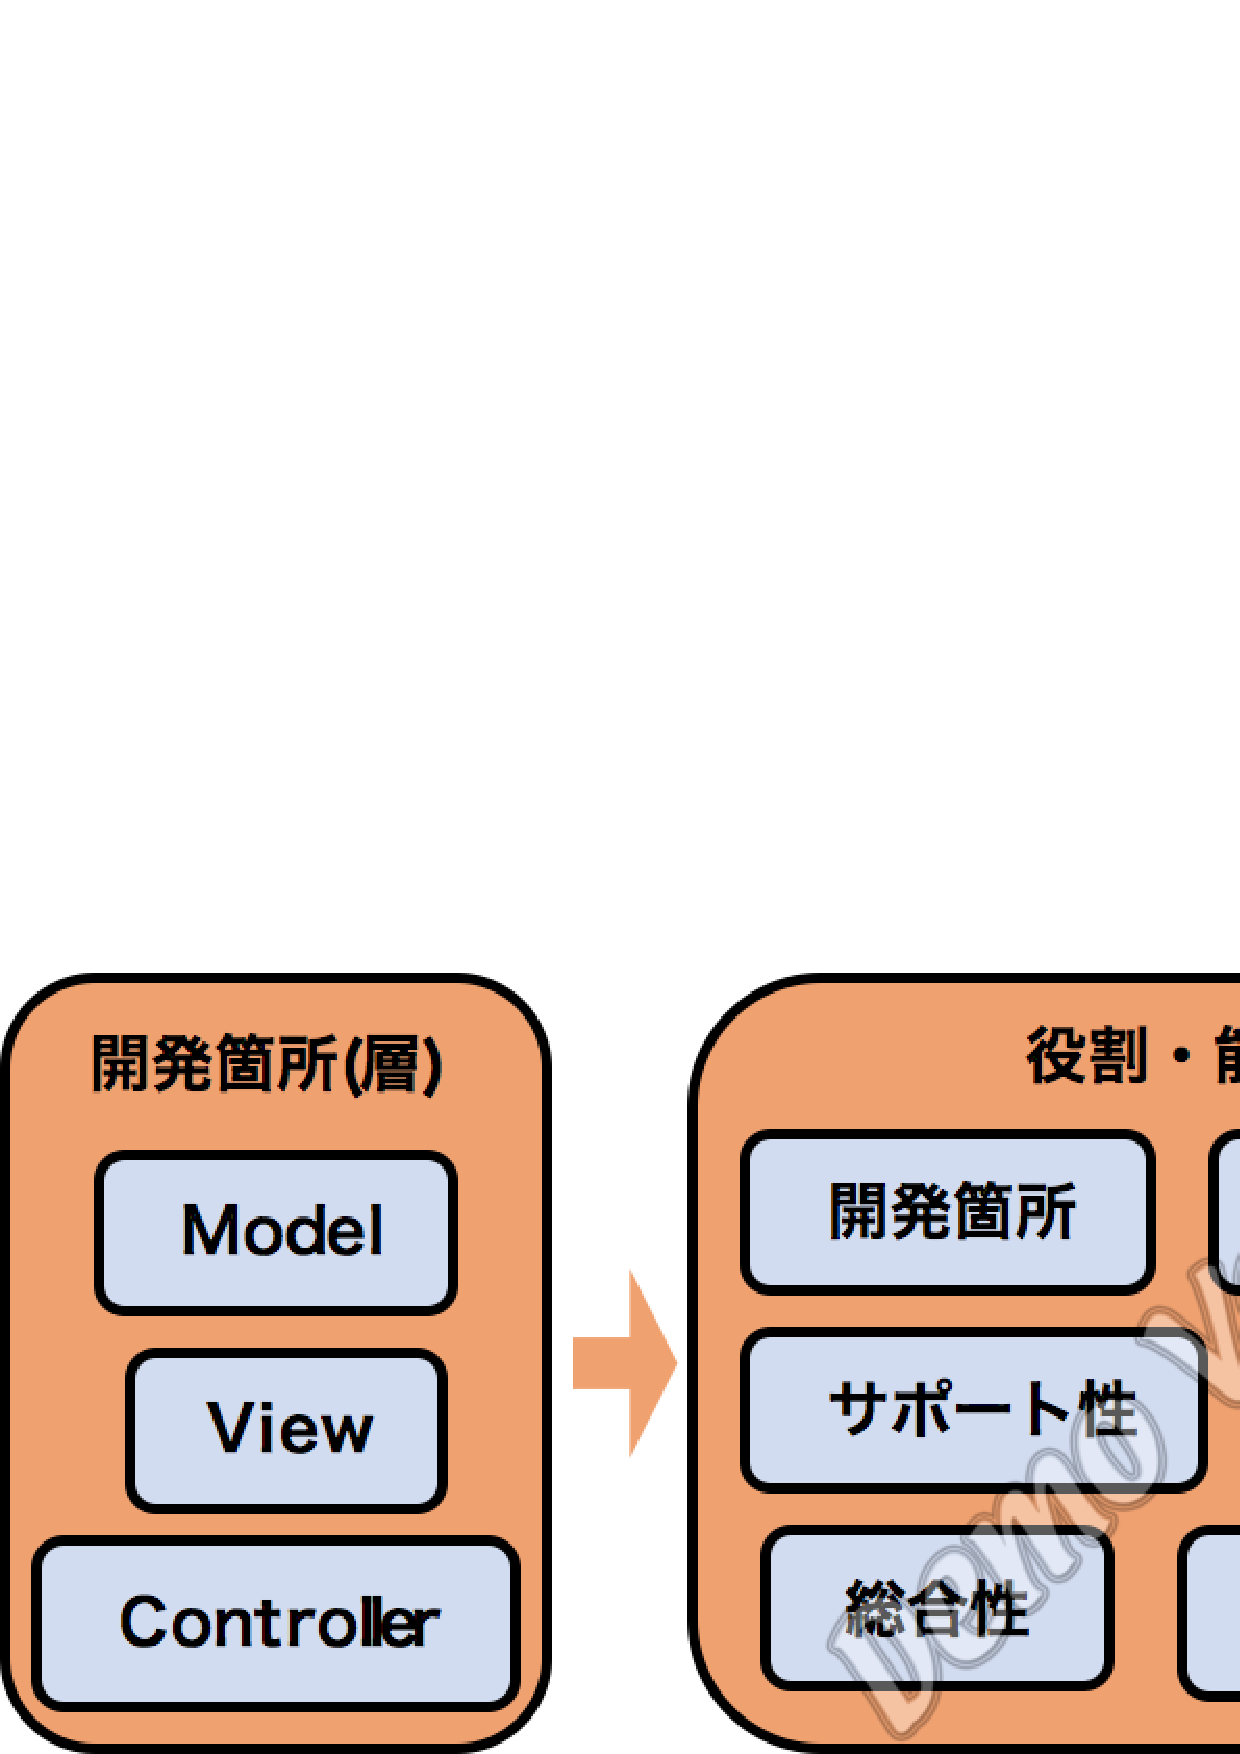
\includegraphics[clip,width=16cm,height=5cm]{figures/overview.pdf}
  \caption{本研究で用いる特徴抽出手法の概要}    \label{sample}
\end{figure}

\section{特徴の算出方法}
本節では,提案手法によるMVCフレームワーク解析に基づいた,開発者の開発箇所,貢献度,サポート性,先導性,総合性の算出方法について述べる.なお,貢献度に関しては李ら\cite{risyo}の関連研究の算出方法を用いて抽出を行う.それ以外の特徴の算出方法は本研究独自の算出方法を用いる.

\subsection{開発役割の抽出}

MVCフレームワークを対象として,View,Model,Controllerの各開発層の作成・修正ファイル数に着目することで役割を抽出する(図4.2).例えば,Controller層の開発が多い開発者は,ロントエンドエンジニアの役割,Model層の開発が多い開発者はデータベースエンジニアの役割を担っている,というように開発箇所から役割の抽出を行う.なお次節以降の算出方法は,この開発箇所ごとによる作成・修正ファイルに応じて適用される.
\begin{figure}[H]
\centering  % 図を真ん中に配置
\includegraphics[clip,width=12cm,height=4cm]{figures/role.pdf}
  \caption{役割の抽出フロー}    \label{sample}
\end{figure}

\subsection{貢献度の抽出}

開発者の貢献度は,質的な貢献度と量的な貢献度に分けて抽出する.
\subsubsection{質的な貢献度}
質的な貢献度は,開発層における重要なモジュール群の開発量に応じて算出する(図4.3).例えば,他の関数からの参照回数が多いライブラリ関数を開発している開発者は,質的な貢献度が高いと考えられる.そこで,参照回数の大い関数の作成数(=a)がしきい値(=μ)より大きい場合,そのライブラリ関数の開発者はプロジェクトの質的な貢献度が高いと判定する(表4.1).

\begin{figure}[H]
\centering  % 図を真ん中に配置
\includegraphics[clip,width=16cm,height=3cm]{figures/contribution_quality.pdf}
  \caption{質的な貢献度の抽出フロー}    \label{sample}
\end{figure}
%%%%%%%%%%%%%%%%%μベータではなくミューを使うよ%%%%%%%%%%%%%%%%%%%%%%%%%%%%%%%%%%
\begin{table}[H]
  \begin{center}
    \begin{tabular}{|c||c|} \hline
      cの範囲 & 貢献値  \\ \hline
      0<a≦μ1 & 1 \\ \hline
      μ1<a≦μ2 & 2 \\ \hline
      μ2<a≦100 & 3  \\ \hline
    \end{tabular}
  \end{center}
  \caption{質的な貢献度のレベル}    \label{sample}
\end{table}

\subsubsection{量的な貢献度}
量的な貢献度は,開発者が作成・修正したソース・ファイル数に応じて算出する.View,Model,Controllerの各層において,新規作成したソース・プログラムおよび他者開発ソース・プログラムを修正した割合(=b)としきい値(=γ)に応じて,量的な貢献度を算出する(表4.2).
\begin{table}[H]
  \begin{center}
    \begin{tabular}{|c||c|} \hline
      bの範囲 & 貢献値  \\ \hline
      0<b≦γ1 & 1 \\ \hline
      γ1<b≦γ2 & 2 \\ \hline
      γ2<b≦100 & 3  \\ \hline
    \end{tabular}
  \end{center}
  \caption{量的な貢献度のレベル}    \label{sample}
\end{table}

\subsection{サポート性の抽出}
%%%%%%%%%%%%%%%%%%%%%εイプシロンの表つくるよ%%%%%%%%%%%%%%%%%%%%%%%%%%
サポート性は,他の開発者への援助の度合いを表す性質であり,他者開発ソース・プログラムのうち,修正したソース・プログラムから算出する.他者開発ファイルの修正数(=c)がしきい値(=ε)以上の際に,その開発者はサポート性があるとする(表4.3).
\begin{table}[H]
  \begin{center}
    \begin{tabular}{|c||c|} \hline
      cの範囲 & サポート性  \\ \hline
      0<c≦ε1 & 1 \\ \hline
      ε1<c≦ε2 & 2 \\ \hline
      ε2<c≦100 & 3  \\ \hline
    \end{tabular}
  \end{center}
  \caption{サポート性のレベル}    \label{sample}
\end{table}

\subsection{先導性の抽出}
%%%%%%%%%%%%%%%%%%%%%%%%%λラムダの表つくるよ%%%%%%%%%%%%%%%%%%%%%%
各開発層における新規ファイルの作成数や,設定ファイル,ライブラリ定義ファイル等,システム環境構築に必要なファイルや・プログラムを率先して作成することは,プロジェクトに参加する他の開発者が効率よく開発進める上で重要である.このため,システム開発に必要なファイルやプログラムのコミット数(=d)がしきい値(=λ)以上の際に,その開発者は先導性が高いと判定する(表4.4).
\begin{table}[H]
  \begin{center}
    \begin{tabular}{|c||c|} \hline
      dの範囲 & 先導性  \\ \hline
      0<d≦λ1 & 1 \\ \hline
      λ1<d≦λ2 & 2 \\ \hline
      λ2<d≦100 & 3  \\ \hline
    \end{tabular}
  \end{center}
  \caption{先導性のレベル}    \label{sample}
\end{table}


\subsection{総合性の抽出}

総合性は,前節で述べたような,各開発層の視点に基づいた貢献性,サポート性,先導性の複合条件によって決定する.条件は対象となるプロジェクトのしきい値(=δ)によって異なるが,例えば貢献性やサポート性と先導性の合計値(=e)が7以上であることを条件とすれば,eが7以上の際に総合性があると判定し,それ以外の場合を総合性が見られなかったという算出結果となる(表4.5).
\begin{table}[H]
  \begin{center}
    \begin{tabular}{|c||c|} \hline
      eの範囲 & 総合性  \\ \hline
      0≦e<δ & false \\ \hline
      δ≦e & true \\ \hline
    \end{tabular}
  \end{center}
  \caption{総合性のレベル}    \label{sample}
\end{table}
%--------------------------------------------------------------------
\chapter{実験と結果}
4章で述べた特徴抽出手法を用いてGitHub上のプロジェクトを対象とした実験を行う.そこで本章では,実験の準備やその対象,実験の方法,そして実験の結果について述べる.
\section{実験準備}
\subsection{実験対象プロジェクト}
GitHubAPIを用いて,GitHub上で公開されている6つのソフトウェア開発プロジェクトを取得した.取得を行う上での条件を下記に示す.
\begin{itemize}
 \item GitHub上でMVCフレームワークRuby on Railsのタグ付けがされていること
 \item Rubyのライブラリやプラグインではなく,Ruby on Railsで開発を行っているプロジェクトであること
 \item プロジェクトのsizeが200MB以下であること
 \item GitHub上でのfork数が上位100位以内であること
\end{itemize}
 以上の4つの条件に合うプロジェクト6つを無作為に選び,実験の対象プロジェクトとした.ここでは6つのそれぞれのプロジェクトをP1〜P6とする.なお,Ruby on Rails\cite{ruby_on_rails}はRuby言語を基とした,Webアプリケーションフレームワークであり,MVCアーキテクチャに基づいて構築されている.今回の実験では,実験を容易に行うために,MVCフレームアーキテクチャを用いているプロジェクトを対象とする.そのため,Ruby on Railsで開発を行なっているプロジェクトを実験対象とする.
\\ ここで,プロジェクトに携わっている開発者のうち,Model層,View層,Controller層のいずれかのファイルに携わっている開発者を分析対象者とする(表5.1).

\begin{table}[htb]
  \begin{center}
    \begin{tabular}{|c||c||c||c|} \hline
      ID & プロジェクト名 & URL & 分析対象人数  \\ \hline
	  P1 & octopub & https://github.com/theodi/octopub & 5名/10名\\ \hline
      P2 & coderdojo.jp & https://github.com/coderdojo-japan/coderdojo.jp & 4名/26名\\ \hline
      P3 & yacs & https://github.com/YACS-RCOS/yacs & 5名/12名\\ \hline
      P4 & poly & https://github.com/wikitongues/poly & 5名/13名\\ \hline
      P5 & hackweek & https://github.com/SUSE/hackweek & 6名/15名\\ \hline
      P6 & where2help & https://github.com/where2help/where2help & 6名/14名\\ \hline    \end{tabular}
  \end{center}
  \caption{分析対象プロジェクト}    \label{sample}
\end{table}
\subsection{実験方法}
本節では前節で述べたプロジェクトP1〜P6の実験の方法を述べる.プロジェクトP1〜P6の各開発者を対象として,5章で提案した手法により,(A)役割,(B)量的な貢献度,(C)質的な貢献度,(D)サポート性,(E)先導性,(F)総合性の抽出を行い,結果を考察する.
\\ (B)のしきい値については,新規ファイル作成率とファイル修正率の合計値が計50%以上の場合にレベル3とし,25〜50%未満の場合にレベル2とし,25%未満の場合にレベル1とした.
(D)や(E)のしきい値に関しても,(B)と同様に新規ファイル作成率とファイル修正率の合計値が計50%以上の場合にレベル3,25〜50%未満の場合にレベル2,25%未満の場合にレベル1とした.
\\ (C)については,各開発層における開発者が開発した関数の中で,最も参照回数が多い関数を開発した開発者をレベル3とし,同様に2番目に参照回数が多い関数を開発した開発者をレベル2とし,それ以外の場合をレベル1とした.ここで,最も参照回数が多い関数が複数あった場合は,それらの関数を開発した開発者をそれぞれレベル3とし,それ以外の開発者をレベル1とする.なお,表5.2はController層に頻繁に利用される関数のリストである.これらの関数はアプリケーションを構成するコンポーネントであり,開発者が作成する関数ではないため,関数の参照回数を調べる際のリストからは除外する.また,View層では関数が使われることが無いに等しいため,View層のみ質的な貢献度の算出は行わない.
\\ 最後に(F)については,Model層とController層では(B)(C)(D)(E)の合計値が8以上の場合に,View層では(B)(D)(E)の合計値が7以上の場合に総合性があると判定する.

\begin{table}[htb]
  \begin{center}
    \begin{tabular}{|c||c|} \hline
      関数名 & 用途  \\ \hline
      index	& すべてのユーザーを表示するページ \\ \hline
      show & id=1のユーザーを表示するページ\\ \hline
      new & ユーザーを新規作成するページ  \\ \hline
      	create & ユーザーを作成するアクション \\ \hline
      edit & id=1のユーザーを編集するページ\\ \hline
      update & id=1のユーザーを更新するアクション \\ \hline
      destroy & id=1のユーザーを削除するアクション \\ \hline
    \end{tabular}
  \end{center}
  \caption{Controller層で自動生成される関数一覧}    \label{sample}
\end{table}

\section{実験結果}
表5.3〜表5.32に,表5.1のプロジェクトP1〜P6を提案手法によって特徴抽出した結果を示す.なお前節で示した通り,View層の質的な貢献度は算出することができないので,「null」と算出される.
\subsection{プロジェクトP1}
表5.3〜表5.5はそれぞれプロジェクトP1におけるModel層,View層,Controller層の解析結果を示している.これらの表は開発者ごとに新規ファイル作成数やファイル修正数,それぞれの割合,そしてその合計値を算出している.例えば表5.3において開発者P1-1はModel層で8つのファイルを新規作成し,4つのファイルを修正している.Model層全体のファイル数が13であるため,それぞれ全体ファイルにおける割合が61.5\%(α)と30.8\%(β)となっている.そしてその割合の合計値が(α+β)が92.3\%と算出されている.また,表5.4と表5.5に関しても表5.3と同様の項目で結果が算出されている.
 \\ また,表5.6はプロジェクトP1に携わる開発者のMVCの各層における開発者の特徴を抽出している.まず,開発者P1-1は表5.7を見ると,Model層やController層において最も算出頻度の高い関数を開発しているため,質的な貢献がレベル3で算出されている.また,その他の算出項目もレベルが高く,表5.6では全ての開発層において総合性がtrueと算出されている.このことから開発者P1-1はプロジェクトP1において開発リーダーという立場であることが考えられる.また,P1-2はView層において,開発者P1-3はView層とControlller層で総合性があると判定されている.このことから,それぞれ開発者P1-2はコーダの役割であり,開発者P1-3はフロントエンドエンジニアの役割であることが考察することができる.また,P1-3は先導性の値に比べ,サポート性の算出結果が高い数値となっている.したがって開発者P1-3はプロジェクトP1において他者をサポートすることが多かったことが考察できる.
%%%%%%%%%%%%%%%P1の各層の算出結果%%%%%%%%%%%
\begin{table}[H]
  \begin{center}
\begin{tabular}{|c|c|c|c|c||c|}\hline
開発者名&作成ファイル数&割合(α)&修正ファイル数&割合(β)&(α)+(β)\\ \hline
P1-1 & 8 & 61.5\% & 4 & 30.8\% & 92.3\%\\ \hline \hline
P1-2 & 4 & 30.8\% & 0 & 30.8\% & 30.8\%\\ \hline \hline
P1-3 & 1 & 7.7\% & 5 & 38.5\% & 46.2\%\\ \hline \hline
P1-4 & 0 & 0\% & 1 & 7.7\% & 7.7\%\\ \hline \hline
P1-5 & 0 & 0\% & 4 & 30.8\% & 30.8\%\\ \hline \hline
\end{tabular}    
\caption{Model層の解析結果(P1)}    \label{sample}
  \end{center}
\end{table}
\begin{table}[H]
  \begin{center}
\begin{tabular}{|c|c|c|c|c||c|}
\hline
開発者名&作成ファイル数&割合(α)&修正ファイル数&割合(β)&(α)+(β)\\ \hline
P1-1 & 31 & 67.4\% & 6 & 13.0\% & 80.4\%\\ \hline \hline
P1-2 & 13 & 28.3\% & 3 & 6.5\% & 34.7\%\\ \hline \hline
P1-3 & 1 & 2.2\% & 24 & 52.2\% & 54.5\%\\ \hline \hline
P1-4 & 1 & 2.2\% & 2 & 4.3\% & 6.5\%\\ \hline \hline
P1-5 & 0 & 0\% & 0 & 0\% & 0\%\\ \hline \hline
\end{tabular}
  \end{center}
  \caption{View層の解析結果(P1)}    \label{sample}
\end{table}
\begin{table}[H]
  \begin{center}
\begin{tabular}{|c|c|c|c|c||c|}
\hline
開発者名&作成ファイル数&割合(α)&修正ファイル数&割合(β)&(α)+(β)\\ \hline
P1-1 & 9 & 69.2\% & 4 & 30.8\% & 100\%\\ \hline \hline
P1-2 & 4 & 30.8\% & 4 & 30.8\% & 61.5\%\\ \hline \hline
P1-3 & 0 & 0\% & 7 & 53.8\% & 53.8\%\\ \hline \hline
P1-4 & 0 & 0\% & 0 & 0\% & 0\%\\ \hline \hline
P1-5 & 0 & 0\% & 4 & 30.8\% & 30/8\%\\ \hline \hline
\end{tabular}
  \end{center}
  \caption{Controller層の解析結果(P1)}    \label{sample}
\end{table}
%%%%%%%%%%%%%%%P1の特徴抽出結果%%%%%%%%%%%%%%%
\begin{table}[H]
  \begin{center}
\begin{tabular}{|c|c|c|c|c|c|c|}
\hline
開発者名 & 役割 & 量的な貢献 & 質的な貢献 & サポート性 & 先導性 & 総合性\\ \hline
& Model & 3 & 3 & 2 & 3 & true\\ \cline{2-7}
P1-1 & View & 3 & null & 1 & 3 & true\\ \cline{2-7}
& Controller & 3 & 3 & 2 & 3 & true \\ \hline \hline

& Model & 2 & 1 & 1 & 2 & false\\ \cline{2-7}
P1-2 & View & 3 & null & 2 & 2 & true\\ \cline{2-7}
& Controller & 2 & 2 & 1 & 2 & flase \\ \hline \hline

& Model & 2 & 2 & 2 & 1 & false\\ \cline{2-7}
P1-3 & View & 3 & null & 3 & 1 & true\\ \cline{2-7}
& Controller & 3 & 1 & 3 & 1 & true \\ \hline \hline

& Model & 1 & 1 & 1 & 1 & false\\ \cline{2-7}
P1-4 & View & 1 & null & 1 & 1 & false\\ \cline{2-7}
& Controller & 1 & 1 & 1 & 1 & false \\ \hline \hline

& Model & 2 & 1 & 2 & 1 & false\\ \cline{2-7}
P1-5 & View & 1 & null & 1 & 1 & false\\ \cline{2-7}
& Controller & 2 & 1 & 2 & 1 & false \\ \hline
\end{tabular}
  \end{center}
  \caption{開発者の特徴抽出結果(P1)}    \label{sample}
\end{table}
%%%%%%%%%%%%%%%参照回数が多い関数の一覧%%%%%%%%%%%%%%%
\begin{table}[H]
  \begin{center}
\begin{tabular}{|c|c|c|c|}\hline
開発層&関数名&参照回数&開発者名\\ \hline
Model& initialize & 9回 & P1-1 \\ \cline{2-4}
& gh\_pager\_url & 8回 & P1-2 \\ \cline{2-4}\hline\hline
Controller& check\_mandatory\_fields & 12回 & P1-1 \\ \cline{2-4}
& user\_params & 8回 & P1-3 \\ \cline{2-4}\hline
\end{tabular}    
\caption{参照回数が多い関数の一覧(P1)}    \label{sample}
  \end{center}
\end{table}
%%%%%%%%%%%%%%%%%%%%%%%%%%%%%%%%%%%%%%プロジェクトP2%%%%%%%%%%%%%%%%%%%%%%%%%%%%%%%%%%%%%%
\subsection{プロジェクトP2}
表5.8〜表5.10はそれぞれプロジェクトP2におけるModel層,View層,Controller層の解析結果を示している.また,表5.11はプロジェクトP2に携わる開発者のMVCの各層における開発者の特徴を抽出している.
\\ Model層(表5.8)とView層(表5.9)の開発層では,修正ファイルの割合が各開発者ともに少ない結果となっている.このことから,プロジェクトP2では新規作成したファイルを他の開発者が修正することが少ないため,1つのファイルを1人が携わるプロジェクト体制であることが考えられる.また,開発者P2-2はView層の全てのファイルを新規作成し,この中のファイルを修正した割合も開発者P2-1の8.1\%と,極めて低い.このため,開発者P2-2はView層で重要な役割を担っていたことがわかる.また,開発者P2-1はController層,開発者P2-3はModel層において総合性があると算出されている.前述の開発者P2-2がView層を担当していたことを含め,MVCの各層において1人ずつメインで開発を行う開発者がいたことが分かる.

\begin{table}[H]
  \begin{center}
\begin{tabular}{|c|c|c|c|c||c|}\hline
開発者名&作成ファイル数&割合(α)&修正ファイル数&割合(β)&(α)+(β)\\ \hline
P2-1 & 5 & 26.3\% & 1 & 5.3\% & 31.6\%\\ \hline \hline
P2-2 & 3 & 15.8\% & 2 & 26.3\% & 26.3\%\\ \hline \hline
P2-3 & 10 & 52.6\% & 0 & 0\% & 52.6\%\\ \hline \hline
P2-4 & 0 & 0\% & 0 & 0\% & 0\%\\ \hline 
\end{tabular}    
\caption{Model層の解析結果(P2)}    \label{sample}
  \end{center}
\end{table}
\begin{table}[H]
  \begin{center}
\begin{tabular}{|c|c|c|c|c||c|}\hline
開発者名&作成ファイル数&割合(α)&修正ファイル数&割合(β)&(α)+(β)\\ \hline
P2-1 & 0 & 0\% & 3 & 8.1\% & 8.1\%\\ \hline \hline
P2-2 & 37 & 100\% & 0 & 0\% & 100\%\\ \hline \hline
P2-3 & 0 & 33.3\% & 0 & 0\% & 0\%\\ \hline \hline
P2-4 & 0 & 0\% & 0 & 0\% & 0\%\\ \hline 
\end{tabular}    
\caption{View層の解析結果(P2)}    \label{sample}
  \end{center}
\end{table}\begin{table}[H]
  \begin{center}
\begin{tabular}{|c|c|c|c|c||c|}\hline
開発者名&作成ファイル数&割合(α)&修正ファイル数&割合(β)&(α)+(β)\\ \hline
P2-1 & 6 & 66.7\% & 3 & 33.3\% & 100\%\\ \hline \hline
P2-2 & 0 & 0\% & 4 & 44.4\% & 44.4\%\\ \hline \hline
P2-3 & 3 & 33.3\% & 0 & 0\% & 33.3\%\\ \hline \hline
P2-4 & 0 & 0\% & 3 & 33.3\% & 33.3\%\\ \hline  
\end{tabular}    
\caption{Controller層の解析結果(P2)}    \label{sample}
  \end{center}
\end{table}
%%%%%%%%%%%%%%%P2の特徴抽出結果%%%%%%%%%%%%%%%
\begin{table}[H]
  \begin{center}
\begin{tabular}{|c|c|c|c|c|c|c|}
\hline
開発者名 & 役割 & 量的な貢献 & 質的な貢献 & サポート性 & 先導性 & 総合性\\ \hline
& Model & 2 & 1 & 1 & 2 & false\\ \cline{2-7}
P2-1 & View & 1 & null & 1 & 1 & false\\ \cline{2-7}
& Controller & 3 & 3 & 1 & 2 & true \\ \hline \hline

& Model & 2 & 2 & 1 & 1 & false\\ \cline{2-7}
P2-2 & View & 3 & null & 1 & 3 & true\\ \cline{2-7}
& Controller & 2 & 1 & 2 & 1 & false \\ \hline \hline

& Model & 3 & 3 & 1 & 3 & true\\ \cline{2-7}
P2-3 & View & 1 & null & 1 & 1 & false\\ \cline{2-7}
& Controller & 2 & 3 & 1 & 2 & false \\ \hline \hline

& Model & 1 & 1 & 1 & 1 & false\\ \cline{2-7}
P2-4 & View & 1 & null& 1 & 1 & false\\ \cline{2-7}
& Controller & 2 & 1 & 2 & 1 & false \\ \hline
\end{tabular}
  \end{center}
  \caption{開発者の特徴抽出結果(P2)}    \label{sample}
\end{table}
%%%%%%%%%%%%%%%P2の参照回数の関数の一覧%%%%%%%%%%%%%%%
\begin{table}[H]
  \begin{center}
\begin{tabular}{|c|c|c|c|}\hline
開発層&関数名&参照回数&開発者名\\ \hline
Model& title & 5回 & P2-3 \\ \cline{2-4}
& path & 4回 & P2-2 \\ \cline{2-4}\hline\hline

& valid\_credentials & 2回 & P2-1 \\ \cline{2-4}
Controller& set\_request\_varian & 2回 & P2-1 \\ \cline{2-4}
& login\_page\_access & 2回 & P2-3 \\ \hline
\end{tabular}    
\caption{参照回数が多い関数の一覧(P2)}    \label{sample}
  \end{center}
\end{table}
%%%%%%%%%%%%%%%%%%%%%%%%%%%%%%%%%%%%%%プロジェクトP3%%%%%%%%%%%%%%%%%%%%%%%%%%%%%%%%%%%%%%
\subsection{プロジェクトP3}
表5.13〜表5.15はそれぞれプロジェクトP3におけるModel層,View層,Controller層の解析結果を示している.また,表5.16はプロジェクトP3に携わる開発者のMVCの各層における開発者の特徴を抽出している.
\\ 表5.13〜表5.15を見ると,MVC各層において新規ファイルを作成した開発者がP3-1とP3-4の2人だけであることが分かる.そのため,その2人の先導性の値が高く,その他の開発者の値はレベル1と算出されている.また総合性の算出結果を見ても,開発者P3-4はModel層とController層において,開発者P3-1は全ての層において総合性があると算出されている.そのため,プロジェクトP3は開発者P3-1と開発者P3-4がメインで開発を行い,その他の開発者がサポート側の役割を担っていたことが分かる.
%%%%%%%%%%%%%%%P3の各層の特徴抽出結果%%%%%%%%%%%%%%%
\begin{table}[H]
  \begin{center}
\begin{tabular}{|c|c|c|c|c||c|}\hline
開発者名&作成ファイル数&割合(α)&修正ファイル数&割合(β)&(α)+(β)\\ \hline
P3-1 & 2 & 50.0\% & 2 & 50.0\% & 100\%\\ \hline \hline
P3-2 & 0 & 0\% & 1 & 25.0\% & 25.0\%\\ \hline \hline
P3-3 & 0 & 0\% & 0 & 0\% & 0\%\\ \hline \hline
P3-4 & 2 & 50.0\% & 1 & 25.0\% & 75.0\%\\ \hline \hline
P3-5 & 0 & 0\% & 1 & 25.0\% & 25.0\%\\ \hline 
\end{tabular}    
\caption{Model層の解析結果(P3)}    \label{sample}
  \end{center}
\end{table}
\begin{table}[H]
  \begin{center}
\begin{tabular}{|c|c|c|c|c||c|}\hline
開発者名&作成ファイル数&割合(α)&修正ファイル数&割合(β)&(α)+(β)\\ \hline
P3-1 & 9 & 69.2\% & 3 & 23.1\% & 92.3\%\\ \hline \hline
P3-2 & 0 & 0\% & 0 & 0\% & 0\%\\ \hline \hline
P3-3 & 0 & 0\% & 0 & 0\% & 0\%\\ \hline \hline
P3-4 & 3 & 23.1\% & 0 & 0\% & 23.1\%\\ \hline \hline
P3-5 & 0 & 0\% & 0 & 0\% & 0\%\\ \hline
\end{tabular}    
\caption{View層の解析結果(P3)}    \label{sample}
  \end{center}
\end{table}\begin{table}[H]
  \begin{center}
\begin{tabular}{|c|c|c|c|c||c|}\hline
開発者名&作成ファイル数&割合(α)&修正ファイル数&割合(β)&(α)+(β)\\ \hline
P3-1 & 3 & 37.5\% & 4 & 25.0\% & 87.5\%\\ \hline \hline
P3-2 & 0 & 0\% & 2 & 25.0\% & 25.0\%\\ \hline \hline
P3-3 & 0 & 0\% & 1 & 12.5\% & 12.5\%\\ \hline \hline
P3-4 & 5 & 62.5\% & 2 & 25.0\% & 87.5\%\\ \hline \hline
P3-5 & 0 & 0\% & 0 & 0\% & 0\%\\ \hline 
\end{tabular}    
\caption{Controller層の解析結果(P3)}    \label{sample}
  \end{center}
\end{table}
%%%%%%%%%%%%%%%P3の特徴抽出結果%%%%%%%%%%%%%%%
\begin{table}[H]
  \begin{center}
\begin{tabular}{|c|c|c|c|c|c|c|}
\hline
開発者名 & 役割 & 量的な貢献 & 質的な貢献 & サポート性 & 先導性 & 総合性\\ \hline

& Model & 3 & 3 & 3 & 3 & true\\ \cline{2-7}
P3-1 & View & 3 & null & 2 & 3 & true\\ \cline{2-7}
& Controller & 3 & 1 & 3 & 2 & true \\ \hline \hline

& Model & 2 & 2 & 2 & 1 & false\\ \cline{2-7}
P3-2 & View & 1 & null & 1 & 1 & false\\ \cline{2-7}
& Controller & 2 & 2 & 2 & 1 & false \\ \hline \hline

& Model & 1 & 1 & 1 & 1 & false\\ \cline{2-7}
P3-3 & View & 1 & null & 1 & 1 & false\\ \cline{2-7}
& Controller & 1 & 1 & 1 & 1 & false \\ \hline \hline

& Model & 3 & 1 & 2 & 3 & true\\ \cline{2-7}
P3-4 & View & 1 & null& 1 & 1 & false\\ \cline{2-7}
& Controller & 3 & 3 & 2 & 3 & true \\ \hline \hline

& Model & 1 & 1 & 2 & 1 & false\\ \cline{2-7}
P3-5 & View & 1 & null & 1 & 1 & false\\ \cline{2-7}
& Controller & 1 & 1 & 1 & 1 & false \\ \hline
\end{tabular}
  \end{center}
  \caption{開発者の特徴抽出結果(P3)}    \label{sample}
\end{table}
%%%%%%%%%%%%%%%P3の参照回数の関数の一覧%%%%%%%%%%%%%%%
\begin{table}[H]
  \begin{center}
\begin{tabular}{|c|c|c|c|}\hline
開発層&関数名&参照回数&開発者名\\ \hline
Model& periods\_changed & 3回 & P3-1 \\ \cline{2-4}
& update\_conflicts & 2回 & P3-2 \\ \cline{2-4}\hline\hline

Controller& any & 5回 & P3-4 \\ \cline{2-4}
& filter & 4回 & P3-2 \\ \cline{2-4}\hline
\end{tabular}    
\caption{参照回数が多い関数の一覧(P3)}    \label{sample}
  \end{center}
\end{table}
%%%%%%%%%%%%%%%%%%%%%%%%%%%%%%%%%%%%%%プロジェクトP4%%%%%%%%%%%%%%%%%%%%%%%%%%%%%%%%%%%%%%
\subsection{プロジェクトP4}
表5.18〜表5.20はそれぞれプロジェクトP4におけるModel層,View層,Controller層の解析結果を示している.また,表5.21はプロジェクトP4に携わる開発者のMVCの各層における開発者の特徴を抽出している.
\\ 表5.21を見ると,開発者P4-1がMVCの各層において総合性があると算出されている.その他の開発者で総合性があると算出されているのは,Controller層での開発者P4-3だけであることから,開発者P4-1がプロジェクト全体の開発をメインで行い,開発者P4-3がController層にて開発者P4-1と同等の活躍をしていたことが分かる.
%%%%%%%%%%%%%%%P4の各層の特徴抽出結果%%%%%%%%%%%%%%%
\begin{table}[H]
  \begin{center}
\begin{tabular}{|c|c|c|c|c||c|}\hline
開発者名&作成ファイル数&割合(α)&修正ファイル数&割合(β)&(α)+(β)\\ \hline
P4-1 & 3 & 75.\% & 1 & 25.0\% & 100\%\\ \hline \hline
P4-2 & 0 & 0\% & 1 & 25.0\% & 25.0\%\\ \hline \hline
P4-3 & 1 & 25.0\% & 0 & 0\% & 25.0\%\\ \hline \hline
P4-4 & 0 & 0\% & 0 & 0\% & 0\%\\ \hline \hline
P4-5 & 0 & 0\% & 1 & 25.0\% & 25.0\%\\ \hline 
\end{tabular}    
\caption{Model層の解析結果(P4)}    \label{sample}
  \end{center}
\end{table}
\begin{table}[H]
  \begin{center}
\begin{tabular}{|c|c|c|c|c||c|}\hline
開発者名&作成ファイル数&割合(α)&修正ファイル数&割合(β)&(α)+(β)\\ \hline
P4-1 & 17 & 100\% & 0 & 0\% & 100\%\\ \hline \hline
P4-2 & 0 & 0\% & 0 & 0\% & 0\%\\ \hline \hline
P4-3 & 0 & 0\% & 2 & 11.8\% & 11.8\%\\ \hline \hline
P4-4 & 0 & 0\% & 0 & 0\% & 0\%\\ \hline \hline
P4-5 & 0 & 0\% & 3 & 17.6\% & 17.6\%\\ \hline 
\end{tabular}    
\caption{View層の解析結果(P4)}    \label{sample}
  \end{center}
\end{table}\begin{table}[H]
  \begin{center}
\begin{tabular}{|c|c|c|c|c||c|}\hline
開発者名&作成ファイル数&割合(α)&修正ファイル数&割合(β)&(α)+(β)\\ \hline
P4-1 & 12 & 92.3\% & 0 & 0\% & 92.3\%\\ \hline \hline
P4-2 & 0 & 0\% & 2 & 15.4\% & 15.4\%\\ \hline \hline
P4-3 & 1 & 7.7\% & 7 & 53.8\% & 61.5\%\\ \hline \hline
P4-4 & 0 & 0\% & 3 & 23.1\% & 23.1\%\\ \hline \hline
P4-5 & 0 & 0\% & 4 & 30.8\% & 30.8\%\\ \hline  
\end{tabular}    
\caption{Controller層の解析結果(P4)}    \label{sample}
  \end{center}
\end{table}
%%%%%%%%%%%%%%%P4の特徴抽出結果%%%%%%%%%%%%%%%
\begin{table}[H]
  \begin{center}
\begin{tabular}{|c|c|c|c|c|c|c|}
\hline
開発者名 & 役割 & 量的な貢献 & 質的な貢献 & サポート性 & 先導性 & 総合性\\ \hline
& Model & 3 & 3 & 2 & 3 & ture\\ \cline{2-7}
P4-1 & View & 3 & null & 1 & 3 & true\\ \cline{2-7}
& Controller & 3 & 3 & 1 & 3 & true \\ \hline \hline

& Model & 2 & 2 & 2 & 1 & false\\ \cline{2-7}
P4-2 & View & 1 & null & 1 & 1 & false\\ \cline{2-7}
& Controller & 1 & 1 & 1 & 1 & false \\ \hline \hline

& Model & 2 & 1 & 1 & 2 & false\\ \cline{2-7}
P4-3 & View & 1 & null& 1 & 1 & false\\ \cline{2-7}
& Controller & 3 & 2 & 3 & 1 & true \\ \hline \hline

& Model & 1 & 1 & 1 & 1 & false\\ \cline{2-7}
P4-4 & View & 1 & null& 1 & 1 & false\\ \cline{2-7}
& Controller & 1 & 1 & 1 & 1 & false \\ \hline \hline

& Model & 2 & 1 & 2 & 1 & false\\ \cline{2-7}
P4-5 & View & 1 & null & 1 & 1 & false\\ \cline{2-7}
& Controller & 2 & 1 & 2 & 1 & false \\ \hline
\end{tabular}
  \end{center}
  \caption{開発者の特徴抽出結果(P4)}    \label{sample}
\end{table}
%%%%%%%%%%%%%%%P4の参照回数の関数の一覧%%%%%%%%%%%%%%%
\begin{table}[H]
  \begin{center}
\begin{tabular}{|c|c|c|c|}\hline
開発層&関数名&参照回数&開発者名\\ \hline
Model& send\_admin\_notification & 5回 & P4-1 \\ \cline{2-4}
& send\_user\_welcome & 3回 & P4-2 \\ \cline{2-4}\hline\hline

& filename & 3回 & P4-1 \\ \cline{2-4}
Controller& presigned\_url & 2回 & P4-1 \\ \cline{2-4}
& favorite & 2回 & P4-3 \\ \hline
\end{tabular}    
\caption{参照回数が多い関数の一覧(P4)}    \label{sample}
  \end{center}
\end{table}
%%%%%%%%%%%%%%%%%%%%%%%%%%%%%%%%%%%%%%プロジェクトP5%%%%%%%%%%%%%%%%%%%%%%%%%%%%%%%%%%%%%%
\subsection{プロジェクトP5}
表5.23〜表5.25はそれぞれプロジェクトP5におけるModel層,View層,Controller層の解析結果を示している.また,表5.26はプロジェクトP5に携わる開発者のMVCの各層における開発者の特徴を抽出している.
\\ 表5.26を見ると,総合性があると算出されているのは開発者P5-1だけである.表5.27にて,開発者P5-2がController層にて質の高い貢献度であることが分かるが,サポート性や先導性の値がレベル1と低く,総合性があると算出されなかった.
%%%%%%%%%%%%%%%P5の各層の特徴抽出結果%%%%%%%%%%%%%%%
\begin{table}[H]
  \begin{center}
\begin{tabular}{|c|c|c|c|c||c|}\hline
開発者名&作成ファイル数&割合(α)&修正ファイル数&割合(β)&(α)+(β)\\ \hline
P5-1 & 7 & 41.2\% & 8 & 47.1\% & 88.2\%\\ \hline \hline
P5-2 & 8 & 47.1\% & 1 & 5.9\% & 52.9\%\\ \hline \hline
P5-3 & 2 & 11.8\% & 0 & 0\% & 11.8\%\\ \hline \hline
P5-4 & 0 & 0\% & 3 & 17.6\% & 17.6\%\\ \hline \hline
P5-5 & 0 & 0\% & 2 & 11.8\% & 11.8\%\\ \hline \hline
P5-6 & 0 & 0\% & 0 & 0\% & 0\%\\ \hline 
\end{tabular}    
\caption{Model層の解析結果(P5)}    \label{sample}
  \end{center}
\end{table}
\begin{table}[H]
  \begin{center}
\begin{tabular}{|c|c|c|c|c||c|}\hline
開発者名&作成ファイル数&割合(α)&修正ファイル数&割合(β)&(α)+(β)\\ \hline
P5-1 & 34 & 79.1\% & 3 & 7.0\% & 86.0\%\\ \hline \hline
P5-2 & 4 & 9.3\% & 1 & 2.3\% & 11.6\%\\ \hline \hline
P5-3 & 1 & 2.3\% & 1 & 2.3\% & 4.6\%\\ \hline \hline
P5-4 & 3 & 7.0\% & 1 & 2.3\% & 9.3\%\\ \hline \hline
P5-5 & 0 & 0\% & 1 & 2.3\% & 2.3\%\\ \hline \hline
P5-6 & 1 & 2.3\% & 2 & 4.6\% & 7.0\%\\ \hline 
\end{tabular}    
\caption{View層の解析結果(P5)}    \label{sample}
  \end{center}
\end{table}\begin{table}[H]
  \begin{center}
\begin{tabular}{|c|c|c|c|c||c|}\hline
開発者名&作成ファイル数&割合(α)&修正ファイル数&割合(β)&(α)+(β)\\ \hline
P5-1 & 8 & 61.5\% & 4 & 30.8\% & 92.3\%\\ \hline \hline
P5-2 & 3 & 23.1\% & 2 & 15.4\% & 38.5\%\\ \hline \hline
P5-3 & 1 & 7.7\% & 1 & 7.7\% & 15.4\%\\ \hline \hline
P5-4 & 0 & 0\% & 3 & 23.1\% & 23.1\%\\ \hline \hline
P5-5 & 1 & 7.7\% & 2 & 15.4\% & 23.1\%\\ \hline \hline
P5-6 & 0 & 0\% & 0 & 0\% & 0\%\\ \hline 
\end{tabular}    
\caption{Controller層の解析結果(P5)}    \label{sample}
  \end{center}
\end{table}
%%%%%%%%%%%%%%%P5の特徴抽出結果%%%%%%%%%%%%%%%
\begin{table}[H]
  \begin{center}
\begin{tabular}{|c|c|c|c|c|c|c|}
\hline
開発者名 & 役割 & 量的な貢献 & 質的な貢献 & サポート性 & 先導性 & 総合性\\ \hline
& Model & 3 & 3 & 2 & 2 & true\\ \cline{2-7}
P5-1 & View & 3 & null & 1 & 3 & true\\ \cline{2-7}
& Controller & 3 & 2 & 2 & 3 & true \\ \hline \hline

& Model & 3 & 1 & 1 & 2 & false\\ \cline{2-7}
P5-2 & View & 1 & null & 1 & 1 & false\\ \cline{2-7}
& Controller & 2 & 3 & 1 & 1 & false \\ \hline \hline

& Model & 1 & 1 & 1 & 1 & false\\ \cline{2-7}
P5-3 & View & 1 & null & 1 & 1 & false\\ \cline{2-7}
& Controller & 1 & 1 & 1 & 1 & false \\ \hline \hline

& Model & 1 & 2 & 1 & 1 & false\\ \cline{2-7}
P5-4 & View & 1 & null& 1 & 1 & false\\ \cline{2-7}
& Controller & 1 & 1 & 1 & 1 & false \\ \hline \hline

& Model & 1 & 1 & 1 & 1 & false\\ \cline{2-7}
P5-5 & View & 1 & null & 1 & 1 & false\\ \cline{2-7}
& Controller & 1 & 1 & 1 & 1 & false \\ \hline \hline

& Model & 1 & 1 & 1 & 1 & false\\ \cline{2-7}
P5-6 & View & 1 & null & 1 & 1 & false\\ \cline{2-7}
& Controller & 1 & 1 & 1 & 1 & false \\ \hline
\end{tabular}
  \end{center}
  \caption{開発者の特徴抽出結果(P5)}    \label{sample}
\end{table}
%%%%%%%%%%%%%%%P5の参照回数の関数の一覧%%%%%%%%%%%%%%%
\begin{table}[H]
  \begin{center}
\begin{tabular}{|c|c|c|c|}\hline
開発層&関数名&参照回数&開発者名\\ \hline
Model& add\_keyword & 12回 & P5-1 \\ \cline{2-4}
& role & 5回 & P5-4 \\ \cline{2-4}\hline\hline

& add\_keyword & 16回 & P5-2 \\ \cline{2-4}
Controller& keyword\_params & 12回 & P5-1 \\ \cline{2-4}
& delete\_keyword & 12回 & P5-2 \\ \cline{2-4}\hline
\end{tabular}    
\caption{参照回数が多い関数の一覧(P5)}    \label{sample}
  \end{center}
\end{table}
%%%%%%%%%%%%%%%%%%%%%%%%%%%%%%%%%%%%%%プロジェクトP6%%%%%%%%%%%%%%%%%%%%%%%%%%%%%%%%%%%%%%
\subsection{プロジェクトP6}
表5.28〜表5.30はそれぞれプロジェクトP6におけるModel層,View層,Controller層の解析結果を示している.また,表5.31はプロジェクトP6に携わる開発者のMVCの各層における開発者の特徴を抽出している.
\\ 表5.28〜表5.30を見ると,Model層の開発者P6-6を除いて,対象の開発者全員がMVC層の全ての層において貢献していることが分かる.その中でも,開発者P6-2がModel層とView層,開発者P6-3がController層にて総合性があると算出されている(表5.31).
%%%%%%%%%%%%%%%P6の各層の特徴抽出結果%%%%%%%%%%%%%%%
\begin{table}[H]
  \begin{center}
\begin{tabular}{|c|c|c|c|c||c|}\hline
開発者名&作成ファイル数&割合(α)&修正ファイル数&割合(β)&(α)+(β)\\ \hline
P6-1 & 1 & 6.7\% & 3 & 20.0\% & 26.7\%\\ \hline \hline
P6-2 & 6 & 40.0\% & 6 & 40.0\% & 80.0\%\\ \hline \hline
P6-3 & 6 & 40.0\% & 1 & 6.7\% & 46.7\%\\ \hline \hline
P6-4 & 1 & 6.7\% & 6 & 40.0\% & 46.7\%\\ \hline \hline
P6-5 & 1 & 6.7\% & 4 & 26.7\% & 33.3\%\\ \hline \hline
P6-6 & 0 & 0\% & 0 & 0\% & 0\%\\ \hline 
\end{tabular}    
\caption{Model層の解析結果(P6)}    \label{sample}
  \end{center}
\end{table}
\begin{table}[H]
  \begin{center}
\begin{tabular}{|c|c|c|c|c||c|}\hline
開発者名&作成ファイル数&割合(α)&修正ファイル数&割合(β)&(α)+(β)\\ \hline
P6-1 & 15 & 33.3\% & 8 & 17.8\% & 51.1\%\\ \hline \hline
P6-2 & 16 & 35.6\% & 11 & 24.4\% & 60.0\%\\ \hline \hline
P6-3 & 4 & 8.9\% & 5 & 11.1\% & 20.0\%\\ \hline \hline
P6-4 & 3 & 6.7\% & 3 & 6.7\% & 13.3\%\\ \hline \hline
P6-5 & 7 & 15.6\% & 14 & 31.1\% & 46.7\%\\ \hline \hline
P6-6 & 0 & 0\% & 1 & 2.2\% & 2.2\%\\ \hline 
\end{tabular}    
\caption{View層の解析結果(P6)}    \label{sample}
  \end{center}
\end{table}\begin{table}[H]
  \begin{center}
\begin{tabular}{|c|c|c|c|c||c|}\hline
開発者名&作成ファイル数&割合(α)&修正ファイル数&割合(β)&(α)+(β)\\ \hline
P6-1 & 8 & 32.0\% & 4 & 16.0\% & 48.0\%\\ \hline \hline
P6-2 & 2 & 8.0\% & 5 & 20.0\% & 28.0\%\\ \hline \hline
P6-3 & 13 & 52.0\% & 7 & 28.0\% & 80.0\%\\ \hline \hline
P6-4 & 2 & 8.0\% & 2 & 8.0\% & 16.0\%\\ \hline \hline
P6-5 & 0 & 0\% & 7 & 28.0\% & 28.0\%\\ \hline \hline
P6-6 & 0 & 0\% & 1 & 2.2\% & 2.2\%\\ \hline 
\end{tabular}    
\caption{Controller層の解析結果(P6)}    \label{sample}
  \end{center}
\end{table}
%%%%%%%%%%%%%%%P6の特徴抽出結果%%%%%%%%%%%%%%%
\begin{table}[H]
  \begin{center}
\begin{tabular}{|c|c|c|c|c|c|c|}
\hline
開発者名 & 役割 & 量的な貢献 & 質的な貢献 & サポート性 & 先導性 & 総合性\\ \hline
& Model & 2 & 3 & 1 & 1 & false\\ \cline{2-7}
P6-1 & View & 3 & null & 1 & 2 & false\\ \cline{2-7}
& Controller & 2 & 1 & 1 & 2 & false \\ \hline \hline

& Model & 3 & 1 & 2 & 2 & true\\ \cline{2-7}
P6-2 & View & 3 & null & 2 & 2 & true\\ \cline{2-7}
& Controller & 2 & 3 & 1 & 1 & false \\ \hline \hline

& Model & 2 & 2 & 1 & 2 & false\\ \cline{2-7}
P6-3 & View & 1 & null & 1 & 1 & false\\ \cline{2-7}
& Controller & 3 & 3 & 2 & 2 & true \\ \hline \hline

& Model & 2 & 1 & 3 & 1 & false\\ \cline{2-7}
P6-4 & View & 1 & null& 1 & 1 & false\\ \cline{2-7}
& Controller & 1 & 1 & 1 & 1 & false \\ \hline \hline

& Model & 2 & 1 & 2 & 1 & false\\ \cline{2-7}
P6-5 & View & 2 & null& 2 & 1 & false\\ \cline{2-7}
& Controller & 1 & 1 & 2 & 1 & false \\ \hline \hline

& Model & 1 & 1 & 1 & 1 & false\\ \cline{2-7}
P6-6 & View & 1 & null & 1 & 1 & false\\ \cline{2-7}
& Controller & 1 & 1 & 1 & 1 & false \\ \hline
\end{tabular}
  \end{center}
  \caption{開発者の特徴抽出結果(P6)}    \label{sample}
\end{table}
%%%%%%%%%%%%%%%P6の参照回数の関数の一覧%%%%%%%%%%%%%%%
\begin{table}[H]
  \begin{center}
\begin{tabular}{|c|c|c|c|}\hline
開発層&関数名&参照回数&開発者名\\ \hline
Model& pending & 14回 & P6-1 \\ \cline{2-4}
& ends\_at & 12回 & P6-3 \\ \cline{2-4}\hline\hline

& opt\_out & 12回 & P6-3 \\ \cline{2-4}
Controller& opt\_in & 12回 & P6-3 \\ \cline{2-4}
& event\_params & 12回 & P6-2 \\ \cline{2-4}\hline
\end{tabular}    
\caption{参照回数が多い関数の一覧(P6)}    \label{sample}
  \end{center}
\end{table}
\section{実験結果のまとめ}
本章は,4章で提案した特徴抽出手法を用いて,表5.1で示したプロジェクトP1〜P6を対象とした実験を行った.提案手法を用いることにより,いずれのプロジェクトも各開発層における貢献値や総合性などの特徴を開発者ごとに抽出することが可能であることが分かった.加えて,算出された数値もも開発者によって分散され,開発者ごとに異なった算出結果となった.また,いずれのプロジェクトも各開発層で総合性がtrueと算出されているのは1~2名に留まり,開発者全員の総合性がtrueもしくはfalseとなるような算出は行われなかった.これらのことから,実験対象人数が4〜6名となる少人数開発プロジェクトでは,実験に用いた算出方法のしきい値は適切であったと考えられる.
%%%%%%%%%%%%%考察のコメントアウト%%%%%%%%%%%%%
\begin{comment}
\chapter{考察}
本章は前章で述べたプロジェクトP1〜P6の特徴抽出結果(表5.3〜表5.8)を基に,それぞれのプロジェクトの考察を述べる.
\section{考察対象}
\subsection{プロジェクトP1}
表5.3を見ると,P1-1が全ての層において総合性がtrueと算出されている.このことからP1-1はプロジェクトP1において開発リーダーという立場であることが考えられる.また,P1-2はView層において,P1-3はView層とController層で総合性があると判定されている.このことから,それぞれP1-2はコーダの役割であり,P1-3はフロントエンドエンジニアの役割であることが考察することができる.また,P1-3は先導性の値に比べ,サポート性の算出結果が高い数値となっている.したがってP1-3はプロジェクトP1において他者をサポートすることが多かったことが考察することができる.
\subsection{プロジェクトP2}
\subsection{プロジェクトP3}
\subsection{プロジェクトP4}
\subsection{プロジェクトP5}
\subsection{プロジェクトP6}
\section{考察まとめ}
\end{comment}
%--------------------------------------------------------------------

%--------------------------------------------------------------------
\chapter{結論と今後の展望}

\section{本研究のまとめ}
近年,ソフトウェア開発における分散バージョン管理システムの普及に伴い,様々なソフトウェア開発プロジェクトがWeb上で共有・管理されるようになっている.本研究では,ソフトウェア開発者の役割や能力などの特徴を抽出することを目的とし,共同開発ツールの代表例であるGitHub上の開発履歴を用いることで,ソフトウェア開発者の特徴抽出手法の提案を行なった.結果として,GitHubのパブリックな6つのプロジェクトを対象とした実験を行い,本提案手法の実現可能性や,その算出結果から分かる考察の可能性があることが分かった.
\section{今後の展望}
本研究では,実験対象人数が少人数(4〜6名)な開発プロジェクトを実験対象としていたため,実験対象人数が10名を超えるような中〜大規模なプロジェクトの実験を行うことで,手法で用いる際のしきい値の適切な値を求めたい.また,複数のプロジェクトにまたがって開発を行なっている開発者を対象としたグローバルな評価を行うことで,より実際の開発状況に適した開発者の特徴抽出手法を拡張していきたい.さらに,提案方式はいわゆる「正解データ」が存在しないため評価が困難である.提案方式の有効性を評価するための方法論の検討を行うことも今後の課題としたい.
%--------------------------------------------------------------------
%%本研究で提案したソフトウェア開発者の特徴抽出手法を現在進行中のプロジェクトに用いることで,プロジェクトマネージャー等のマネジメントを行う立場のユーザーや,プロジェクトの開発者にどのような効果が現れるか,検証を行いたい.
%--------------------------------------------------------------------
\chapter*{謝辞}

本研究において、本学伊藤恵先生には,お忙しい中,研究に関する助言をしていただきました.ここに深く感謝申し上げます.また,伊藤研究室の皆様,その他研究に関するアドバイスをしていただいた方に深く感謝いたします.
%--------------------------------------------------------------------
% 参考文献
\begin{thebibliography}{20}
 \bibitem {GitHub} Github, https://github.com[2018/01/26].
 \bibitem {Onoue_English} Onoue, S., Hata, H. and Matsumoto,K.: A Study of the Characteristics of Developers Activities in Github, Proc.IWESEP ’13, pp.7–12 (2013).
 \bibitem{GitHub_API} GitHub API v3, https://developer.github.com/v3/[2018/01/26].
 \bibitem{Characteristic}Exploring Expressions of Emotions in GitHub Commit Messages,
\\ http://geeksta.net/geeklog/exploring-expressions-emotions-github-commit-messages/[2018/01/26].
 \bibitem{Matsubara} 松原 克弥,伊藤 恵,木塚 あゆみ,コード管理ツールGitを活用した分散PBLにおけるチーム活動過程の可視化の試み, 2016.
 \bibitem{Onoue_Japan} 尾上 紗野, 畑 秀明, 松本健一, GitHub上の活動履歴分析による開発者分類, 情報処理学会論文誌, Vol.56-2-715-719, 2015.
 \bibitem{risyo} 李 書, 鷹野 孝典,分散バージョン管理システムの共同開発履歴に基づいた開発者の特徴抽出手法の検討,情報処理学会研究報告,2015-162-1(1), pp.1-8, 2015.
 \bibitem{gota}五田 篤志, 山崎 尚, 玉田 春昭, 畑 秀明, 角田 雅照, 井垣 宏, 開発履歴を利用した風林火山モデルに基づく開発者特性の分析, 2014-SE-185.
 \bibitem{google_trends}Google Tredns, https://trends.google.co.jp/trends/explore?date=all\&q=Git,Subversion[2018/01/26].
\bibitem{ruby_on_rails} Ruby on Rails, http://rubyonrails.org/[2018/01/26].
\end{thebibliography}


% 以降,付録(付属資料)であることを示す
\appendix
\begin{comment}
%--------------------------------------------------------------------
\chapter*{付録その1} % \chapter{}を使うと「付録A ***」となる

付録その1(プログラムのソースリストなど)を必要があれば載せる
\end{comment}
%--------------------------------------------------------------------
\begin{comment}
\chapter*{付録その2}

付録その2(関連資料など)を必要があれば載せる
\end{comment}

%--------------------------------------------------------------------
% 図一覧
\listoffigures

%--------------------------------------------------------------------
% 表一覧
\listoftables

\end{document}
